\appendix
\chapter*{Приложение А}
\addcontentsline{toc}{chapter}{Приложение А}

Пример сгенерированного кода на octave:
\linespread{1} % вернем временно единичный межстрочный интервал
\lstinputlisting{octave.m}
\begin{figure}[ht]
  \begin{adjustbox}{addcode={\begin{minipage}{\width}}{\caption{%
      Блок-схема подстройки параметров жадного алгоритма ч.1
      } \end{minipage}},rotate=270,center}

  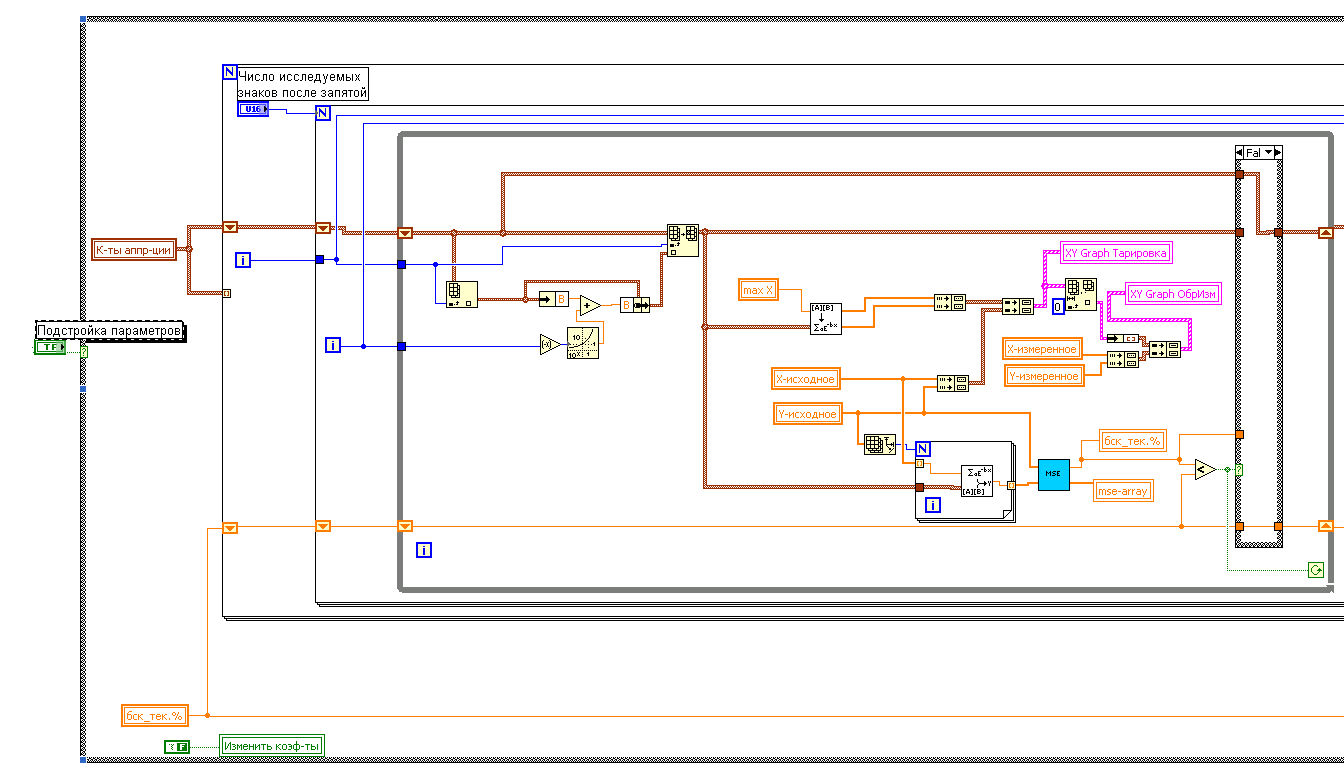
\includegraphics [scale=0.75] {Block-Schema1} 
  \end{adjustbox}
\end{figure}


\begin{figure}[t]
  \begin{adjustbox}{addcode={\begin{minipage}{\width}}{\caption{%
      Блок-схема подстройки параметров жадного алгоритма ч.2
      } \end{minipage}},rotate=270,center}

  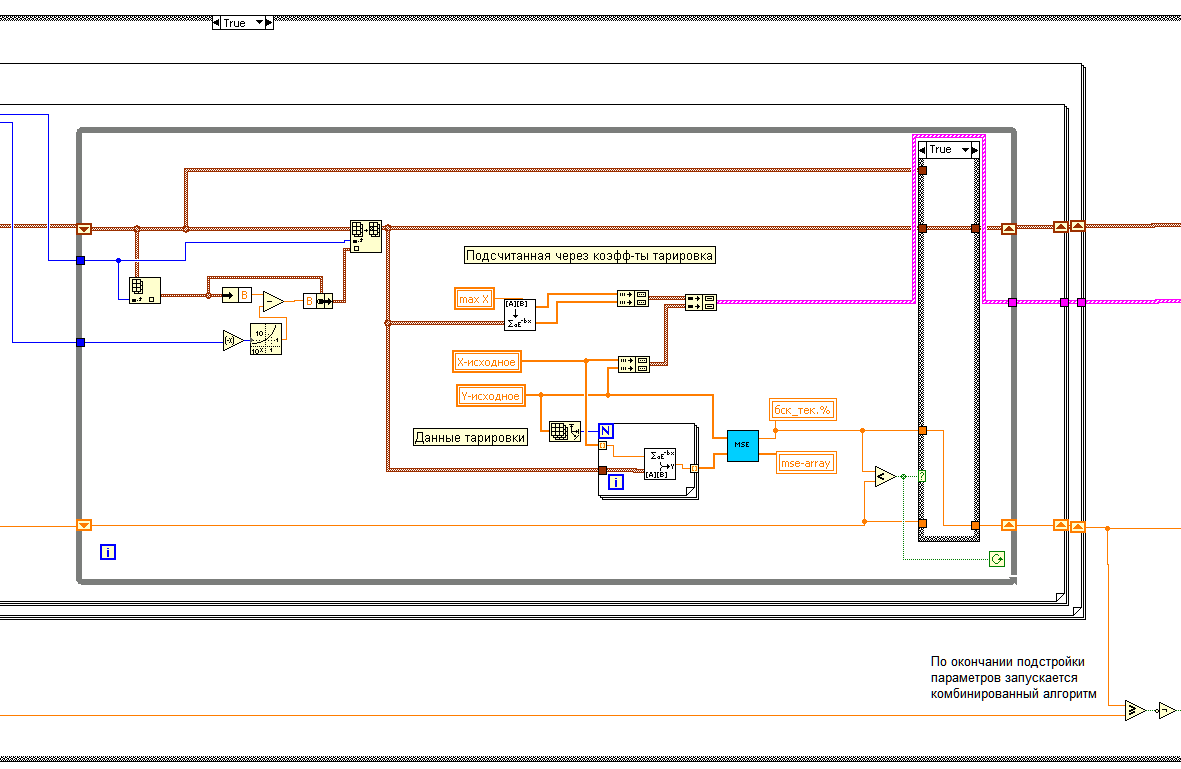
\includegraphics [scale=0.75] {Block-Schema2} 
  \end{adjustbox}
\end{figure}
\begin{figure}[t]
  \begin{adjustbox}{addcode={\begin{minipage}{\width}}{\caption{%
      Блок-схема подстройки параметров жадного алгоритма ч.3
      } \end{minipage}},rotate=270,center}

  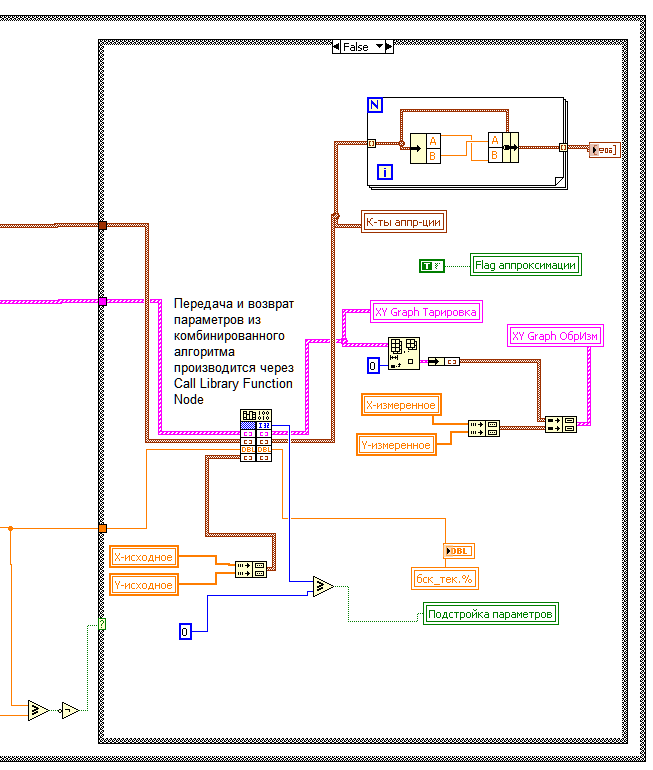
\includegraphics [scale=0.75] {Block-Schema3} 
  \end{adjustbox}
\end{figure}

\lstset{ %
  language=C++
}

Часть динамической библиотеки, отвечающей за связывание кода написанного на языках octave и LabVIEW:
\lstinputlisting{dll_combined.cpp}
%
%Некоторый текст.
%
%\chapter{Очень длинное название второго приложения, в котором продемонстрирована работа с длинными таблицами} \label{AppendixB}

% \section{Подраздел приложения}\label{AppendixB1}
%Вот размещается длинная таблица:
%\fontsize{10pt}{10pt}\selectfont
%\begin{longtable}[c]{|l|c|l|l|}
% \caption{Описание входных файлов модели}\label{Namelists} 
%\\ 
% \hline
 %\multicolumn{4}{|c|}{\textbf{Файл puma\_namelist}}        \\ \hline
% Параметр & Умолч. & Тип & Описание               \\ \hline
%                                              \endfirsthead   \hline
% \multicolumn{4}{|c|}{\small\slshape (продолжение)}        \\ \hline
% Параметр & Умолч. & Тип & Описание               \\ \hline
%                                              \endhead        \hline
% \multicolumn{4}{|r|}{\small\slshape продолжение следует}  \\ \hline
%                                              \endfoot        \hline
%                                              \endlastfoot
% \multicolumn{4}{|l|}{\&INP}        \\ \hline 
% kick & 1 & int & 0: инициализация без шума ($p_s = const$) \\
%      &   &     & 1: генерация белого шума                  \\
%      &   &     & 2: генерация белого шума симметрично относительно \\
%  & & & экватора    \\
% mars & 0 & int & 1: инициализация модели для планеты Марс     \\
% kick & 1 & int & 0: инициализация без шума ($p_s = const$) \\
%      &   &     & 1: генерация белого шума                  \\
%      &   &     & 2: генерация белого шума симметрично относительно \\
%  & & & экватора    \\
% mars & 0 & int & 1: инициализация модели для планеты Марс     \\
%kick & 1 & int & 0: инициализация без шума ($p_s = const$) \\
%      &   &     & 1: генерация белого шума                  \\
%      &   &     & 2: генерация белого шума симметрично относительно \\
%  & & & экватора    \\
% mars & 0 & int & 1: инициализация модели для планеты Марс     \\
%kick & 1 & int & 0: инициализация без шума ($p_s = const$) \\
%      &   &     & 1: генерация белого шума                  \\
%      &   &     & 2: генерация белого шума симметрично относительно \\
%  & & & экватора    \\
% mars & 0 & int & 1: инициализация модели для планеты Марс     \\
%kick & 1 & int & 0: инициализация без шума ($p_s = const$) \\
%      &   &     & 1: генерация белого шума                  \\
%      &   &     & 2: генерация белого шума симметрично относительно \\
%  & & & экватора    \\
% mars & 0 & int & 1: инициализация модели для планеты Марс     \\ 
% \hline 
%\end{longtable}

%\fontsize{14pt}{15pt}\selectfont
%\section{Ещё один подраздел приложения} \label{AppendixB2}

%Нужно больше подразделов приложения!

%\section{Очередной подраздел приложения} \label{AppendixB3}

%Нужно больше подразделов приложения!

%\section{И ещё один подраздел приложения} \label{AppendixB4}

%Нужно больше подразделов приложения!

